\documentclass[aspectratio = 169]{beamer}

\usepackage[utf8]{inputenc}
%\usepackage[utf8]{inputenc}

%%%%%%%% The beamer Theme %%%%%%%%%%%%%%%%%%%%%%
\usetheme{Rochester}
%\usetheme{metropolis}
%\usepackage[dvipdfmx]{graphicx}
\setbeamertemplate{navigation symbols}{}
%\usecolortheme{seagull}
%\usecolortheme{dove}
%\usecolortheme{owl}

%フラットデザインにする
\setbeamertemplate{blocks}[rounded] % Blockの影を消す
\useinnertheme{circles} % 箇条書きをシンプルに
\setbeamertemplate{navigation symbols}{} % ナビゲーションシンボルを消す
%\setbeamertemplate{headline}{}    %フレームタイトルの背景の色を消す
\setbeamertemplate{footline}[frame number] % フッターはスライド番号のみ
\renewcommand{\baselinestretch}{1.2}

%Beamerフォント設定
%\usepackage[]{cmbright} %% Option 'defaultfam'
%% only if the base font of the document is to be sans serig
%\renewcommand*\oldstylenums[1]{{\fontfamily{Montserrat-TOsF}\selectfont #1}}

%\usepackage{newtxtext,newtxmath} % TXフォント
%\usepackage{sfmath}
%\usepackage[deluxe,uplatex]{otf} % 日本語多ウェイト化
%\renewcommand{\familydefault}{\sfdefault}  % 英文をサンセリフ体に
%\DeclareSymbolFont{operators}{OT1}{\sfdefault}{m}{n}
%\SetSymbolFont{operators}{bold}{OT1}{\sfdefault}{b}{n}
%\usepackage{mathrsfs}   %数式の文字をセリフに変える
%\usefonttheme{structurebold} % タイトル部を太字
%\setbeamerfont{alerted text}{series=\bfseries} % Alertを太字
%\setbeamerfont{section in toc}{series=\mdseries} % 目次は太字にしない
%\setbeamerfont{frametitle}{size=\Large} % フレームタイトル文字サイズ
%\setbeamerfont{title}{size=\LARGE} % タイトル文字サイズ
%\setbeamerfont{date}{size=\small}  % 日付文字サイズ

%%%%%%%%%%%%%% Packages %%%%%%%%%%%%%%%%%%%%%%
\usepackage{tikz}
\usepackage{bm}
\usepackage{natbib} % For reference https://gking.harvard.edu/files/natnotes2.pdf
\usepackage{multirow}
\usepackage{setspace}
\usepackage{booktabs}
\usepackage{caption}
\usepackage{subcaption}

%%%%%%%%%%%%%%  Math Environment %%%%%%%%%%%%%% 
\usepackage{amsmath}
\usepackage{amsbsy}
\usepackage{ascmac}
\usepackage{amsthm}
\usepackage{amssymb}
\usepackage{mathtools}

%%%%%%% Theorem Environment based on amsthm %%%%%%%%%%%%%
\theoremstyle{definition}
\setbeamertemplate{theorems}[numbered] 
\newtheorem{thm}{Theorem}
\newtheorem{assm}{Assumption}
\newtheorem{lmma}{Lemma}
\newtheorem{prop}{Proposition}
\newtheorem{rslt}{Result}
\newtheorem{dfn}{Definition}
\newtheorem{crll}{Corollary}

\newtheorem{thm*}{Theorem}
\newtheorem{assm*}{Assumption}
\newtheorem{lmma*}{Lemma}
\newtheorem{prop*}{Proposition}
\newtheorem{rslt*}{Result}
\newtheorem{dfn*}{Definition}
\newtheorem{crll*}{Corollary}


%%%%%%%%%%%%%%%%%%%%%%%%%%%%%% User specified LaTeX commands.
\newcommand{\indep}{\perp \!\!\! \perp}
\newcommand{\argmax}{\operatornamewithlimits{arg\ max}}
\newcommand{\argmin}{\operatornamewithlimits{arg\ min}}


\title{Conduct Parameter Estimation}
%\subtitle{Backus, Conlon, and Sinkinson, Working Paper, 2021}
\author{Yuri Matsumura}
\date{\today}

\begin{document}

\maketitle

\section{Conduct parameter estimation}
\begin{frame}{Conduct parameter estimation}
    \begin{itemize}
        \item Measuring competitiveness in markets is an important task in Empirical industrial organization
        \item Conduct parameter is regarded as a useful measure of competitiveness
        \item In homogeneous product market, the market aggregate supply relation is given as
        \begin{align*}
            P_t = -\theta_{t}\frac{\partial P_t}{\partial Q_t}Q_t + MC_t(Q_t),
        \end{align*}
        where $\theta_t$ is the conduct parameter
        \item When $\theta = 1$, the supply relation represents collusion, $\theta = 1/N$ represents Cournot, $\theta =0$ represents perfect competitive market
    \end{itemize}
\end{frame}

\begin{frame}{}
    \begin{itemize}
        \item Bresnahan (1982) and Lau(1982) consider the identification of $\theta$
        \item Bresnahan (1982) considers a linear demand and linear marginal cost model:
        \begin{align}
            P_t &= \alpha_0 - (\alpha_1 + \alpha_2Z^{R}_{t})Q_t + \alpha_3 Y_t + \varepsilon^{d}_{t},\label{eq:linear_demand}\\
            MC_t &= \gamma_0  + \gamma_1 Q + \gamma_2 W_{t} + \gamma_3 R_t + \varepsilon^{c}_{t},\label{eq:linear_marginal_cost}.
        \end{align}
        \item In this case, the supply relation is written as
        \begin{align}
            P_t = \gamma_0 + [\theta(\alpha_1 + \alpha_2Z^{R}_{t})+ \gamma_1] Q_t   + \gamma_2 W_{t} + \gamma_3 R_t + \varepsilon^{c}_{t}\label{eq:linear_supply_equation}
        \end{align}
        \item As the demand parameter $\alpha$ can be separately identified, we can also identify the conduct and marginal cost parameter
    \end{itemize}
\end{frame}

\begin{frame}{}
    \begin{itemize}
        \item Perloff and Shen (2012) show that when the error terms in the demand and marginal cost equation are both zero, due to the multicollinearity problem, we can not estimate the model
        \item When the standard deviation of the error terms is small, they claim that the nearly perfect collinearity problem occurs
        \item To see the effect of nearly perfect collinearity problem, Perloff and Shen (2012) conduct simulations
        \item Based on their simulation studies, Perloff and Shen (2012) concludes that the researchers can not accurately estimate the conduct parameter
        
    \end{itemize}
\end{frame}

\begin{frame}{}
    \begin{itemize}
        \item However, their simulation has some problems
        \begin{itemize}
            \item Their simulation does not include any demand shifter for the supply estimation
            \item It considers only one sample size in each simulation ($n = 50$) 
        \end{itemize}
        \item We reinvestigate their simulation model
        \item We find that the researchers accurately estimate the conduct parameter by properly adding demand shifters to the supply estimation
        \item Increasing sample size also increases the accuracy of the estimation
    \end{itemize}
\end{frame}

\begin{frame}{Simulation setting}
    \begin{itemize}
        \item We generate 1000 simulation data sets
        \item The parameter setting is the same with Perloff and Shen (2012)
        \item Perloff and Shen (2012) does not include a demand shfter $Y_t$
        \item The estimation of the demand and supply equation are done separately and we apply the 2SLS for each equation
        \item We also change the market size in each simulation, although Perloff and Shen (2012) only consider $n = 50$
    \end{itemize}
\end{frame}

\begin{frame}{Result}
    \begin{table}[]
        \centering
        \tiny
\begin{tabular}[t]{lrrrrrrrr}
\toprule
  & (1) $n=50$ / Mean & (1) $n=50$ / SD & (2) $n=100$ / Mean & (2) $n=100$ / SD & (3) $n=200$ / Mean & (3) $n=200$ / SD & (4) $n=1000$ / Mean & (4) $n=1000$ / SD\\
\midrule
$\alpha_{0}$ & 10.000 & 0.0009 & 10.000 & 0.0007 & 10.000 & 0.0004 & 10.000 & 0.0002\\
$\alpha_{1}$ & 1.000 & 0.004 & 1.000 & 0.003 & 1.000 & 0.002 & 1.000 & 0.0009\\
$\alpha_{2}$ & 1.000 & 0.0005 & 1.000 & 0.0003 & 1.000 & 0.0002 & 1.000 & 0.0001\\
$\alpha_{3}$ & 1.000 & 0.0002 & 1.000 & 0.0001 & 1.000 & 0.0001 & 1.000 & 0.00004\\
$\gamma_{0}$ & 1.000 & 0.001 & 1.000 & 0.001 & 1.000 & 0.0007 & 1.000 & 0.0003\\
$\gamma_{1}$ & 1.000 & 0.005 & 1.000 & 0.004 & 1.000 & 0.002 & 1.000 & 0.001\\
$\gamma_{2}$ & 1.000 & 0.0002 & 1.000 & 0.0001 & 1.000 & 0.0001 & 1.000 & 0.00004\\
$\gamma_{3}$ & 1.000 & 0.0002 & 1.000 & 0.0002 & 1.000 & 0.0001 & 1.000 & 0.00005\\
$\theta$ & 0.500 & 0.0006 & 0.500 & 0.0004 & 0.500 & 0.0003 & 0.500 & 0.0001\\
$R^{2}$ (demand) & 1.000 & 0.0000003 & 1.000 & 0.0000002 & 1.000 & 0.0000002 & 1.000 & 7e-08\\
$R^{2}$ (supply) & 1.000 & 0.0000003 & 1.000 & 0.0000002 & 1.000 & 0.0000002 & 1.000 & 7e-08\\
Sample size ($T$) &  & 50 &  & 100 &  & 200 &  & 1000\\
\bottomrule
\end{tabular}

        \caption{The estimation without demand shfter. $\theta_0 = 0.5$. All true $\gamma$ are one. $\sigma = 0.001$}
        \label{tab:linear_without_demand}
    \end{table}
\end{frame}



\begin{frame}{Result}
    \begin{table}[]
        \centering
        \tiny
\begin{tabular}[t]{lrrrrrrrr}
\toprule
  & Mean & SD & Mean  & SD  & Mean   & SD   & Mean    & SD   \\
\midrule
$\alpha_{0}$ & 9.515 & 6.752 & 9.912 & 1.479 & 9.987 & 0.943 & 9.987 & 0.396\\
$\alpha_{1}$ & 0.362 & 19.344 & 0.710 & 6.192 & 1.154 & 4.363 & 0.986 & 1.728\\
$\alpha_{2}$ & 0.934 & 1.092 & 1.004 & 0.743 & 0.981 & 0.494 & 0.998 & 0.204\\
$\gamma_{0}$ & 5.658 & 6.892 & 5.464 & 8.387 & 5.695 & 8.243 & 5.572 & 10.796\\
$\gamma_{1}$ & 0.956 & 52.166 & 1.715 & 42.062 & -0.056 & 11.467 & 0.388 & 3.140\\
$\gamma_{2}$ & 0.479 & 0.827 & 0.496 & 0.907 & 0.486 & 0.902 & 0.497 & 1.185\\
$\theta$ & -0.296 & 5.941 & -0.439 & 5.106 & -0.235 & 2.034 & -0.256 & 1.771\\
$R^{2}$ (demand) & -3.456 & 87.362 & -0.513 & 1.557 & -0.436 & 0.563 & -0.376 & 0.185\\
$R^{2}$ (supply) & -1.104 & 5.881 & -2.311 & 26.606 & -1.993 & 26.973 & -3.591 & 49.060\\
Sample size ($T$) &  & 50 &  & 100 &  & 200 &  & 1000\\
\bottomrule
\end{tabular}

        \caption{The estimation without demand shfter. $\theta_0 = 0.5$. All true $\gamma$ are one. $\sigma = 2.0$}
        \label{tab:linear_without_demand}
    \end{table}
\end{frame}




\begin{frame}{Log-linear model}
    \begin{itemize}
        \item Perloff and Shen (2012) claims that to solve the multicollinearity and nearly perfect collinearity problem, the log-linear demand and the log-linear model is a better specification for estimating the conduct parameter
        \begin{align}
            \log P_{t} &= \alpha_0 - (\alpha_1 + \alpha_2 Z^{R}_{t}) \log Q_t + \alpha_3 \log Y_t + \varepsilon^{d}_{t},\label{eq:log_linear_demand}\\
            \log MC_t &= \gamma_0 + \gamma_1 \log Q_t +  \gamma_2 \log W_{t} + \gamma_3 \log R_t + \varepsilon^{c}_{t}.\label{eq:log_linear_marginal_cost}
        \end{align}
        \item We also investigate the log-linear model and find that the model faces other problems in estimation
    \end{itemize}
\end{frame}

\begin{frame}{Simulation setting}
    \begin{itemize}
        \item We also generate 1000 data sets and separately estimate the demand and supply equations
        \item As the demand equation is linear, we apply the 2SLS as in the linear model
        \item The supply equation is nonlinear and we apply the GMM
        \item We solve the minimization problem by using a nonlinear solve \texttt{IPOPT}
    \end{itemize}
\end{frame}


\begin{frame}{}
        \begin{table}[]
        \centering
        \tiny
\begin{tabular}[t]{lrrrrrrrr}
\toprule
  & Mean & SD & Mean  & SD  & Mean   & SD   & Mean    & SD   \\
\midrule
$\alpha_{0}$ & 10.000 & 0.004 & 9.998 & 0.004 & 10.001 & 0.002 & 10.000 & 0.001\\
$\alpha_{1}$ & 1.000 & 0.001 & 0.999 & 0.001 & 1.000 & 0.000 & 1.000 & 0.000\\
$\alpha_{2}$ & 0.100 & 0.000 & 0.100 & 0.000 & 0.100 & 0.000 & 0.100 & 0.000\\
$\alpha_{3}$ & 1.000 & 0.000 & 1.000 & 0.000 & 1.000 & 0.000 & 1.000 & 0.000\\
$\gamma_{0}$ & 1.001 & 0.007 & 1.003 & 0.004 & 0.999 & 0.003 & 1.000 & 0.001\\
$\gamma_{1}$ & 1.000 & 0.001 & 1.000 & 0.001 & 1.000 & 0.000 & 1.000 & 0.000\\
$\gamma_{2}$ & 1.000 & 0.001 & 1.000 & 0.000 & 1.000 & 0.000 & 1.000 & 0.000\\
$\gamma_{3}$ & 1.000 & 0.001 & 1.000 & 0.000 & 1.000 & 0.000 & 1.000 & 0.000\\
$\theta$ & 0.098 & 0.004 & 0.099 & 0.002 & 0.100 & 0.002 & 0.100 & 0.001\\
Runs converged (\%) &  & 100.000 &  & 100.000 &  & 100.000 &  & 100.000\\
Sample size ($T$) &  & 50 &  & 100 &  & 200 &  & 1000\\
\bottomrule
\end{tabular}

        \caption{The estimation without demand shfter. $\theta_0 = 0.5$. All true $\gamma$ are one, $\sigma = 0.001$}
        \label{tab:linear_without_demand}
    \end{table}
\end{frame}


\begin{frame}{}
        \begin{table}[]
        \centering
        \tiny
\begin{tabular}[t]{lrrrrrrrr}
\toprule
  & Mean & SD & Mean  & SD  & Mean   & SD   & Mean    & SD   \\
\midrule
$\alpha_{0}$ & 6.416 & 10.448 & 7.385 & 8.342 & 8.366 & 6.582 & 9.953 & 2.371\\
$\alpha_{1}$ & 0.206 & 2.362 & 0.419 & 1.840 & 0.637 & 1.484 & 0.991 & 0.529\\
$\alpha_{2}$ & 0.054 & 0.458 & 0.073 & 0.285 & 0.077 & 0.161 & 0.097 & 0.060\\
$\alpha_{3}$ & 0.613 & 1.169 & 0.699 & 1.287 & 0.824 & 0.713 & 0.996 & 0.270\\
$\gamma_{0}$ & 3.496 & 10.722 & 3.919 & 8.277 & 3.947 & 6.162 & 3.213 & 4.890\\
$\gamma_{1}$ & 1.153 & 1.890 & 1.140 & 1.282 & 1.038 & 0.384 & 1.008 & 0.153\\
$\gamma_{2}$ & 1.098 & 1.669 & 1.003 & 0.762 & 1.007 & 0.526 & 0.998 & 0.233\\
$\gamma_{3}$ & 1.070 & 0.933 & 1.065 & 0.938 & 1.008 & 0.271 & 1.002 & 0.114\\
$\theta$ & -492931.516 & 3240081.766 & -323566.285 & 3240305.105 & -126662.656 & 605408.511 & -15515.297 & 50597.540\\
Solved (%) &  & 0.326 &  & 0.354 &  & 0.389 &  & 0.498\\
Sample size (n) &  & 50 &  & 100 &  & 200 &  & 1000\\
\bottomrule
\end{tabular}

        \caption{The estimation without demand shfter. $\theta_0 = 0.5$. All true $\gamma$ are one, $\sigma = 2.0$}
        \label{tab:linear_without_demand}
    \end{table}
\end{frame}

\begin{frame}{}
    \begin{itemize}
        \item The estimation of the conduct parameter is inaccurate and we can see many negative values which are not theoretically supported
        \item The inaccuracy comes from the relationship between the conduct parameter and the constant term in the marginal cost equation
        \item The contour map of the GMM objective function with respect to $\theta$ and $\gamma_0$ has a flat region
    \end{itemize}
\end{frame}

\begin{frame}{}
    \begin{figure}
        \centering
        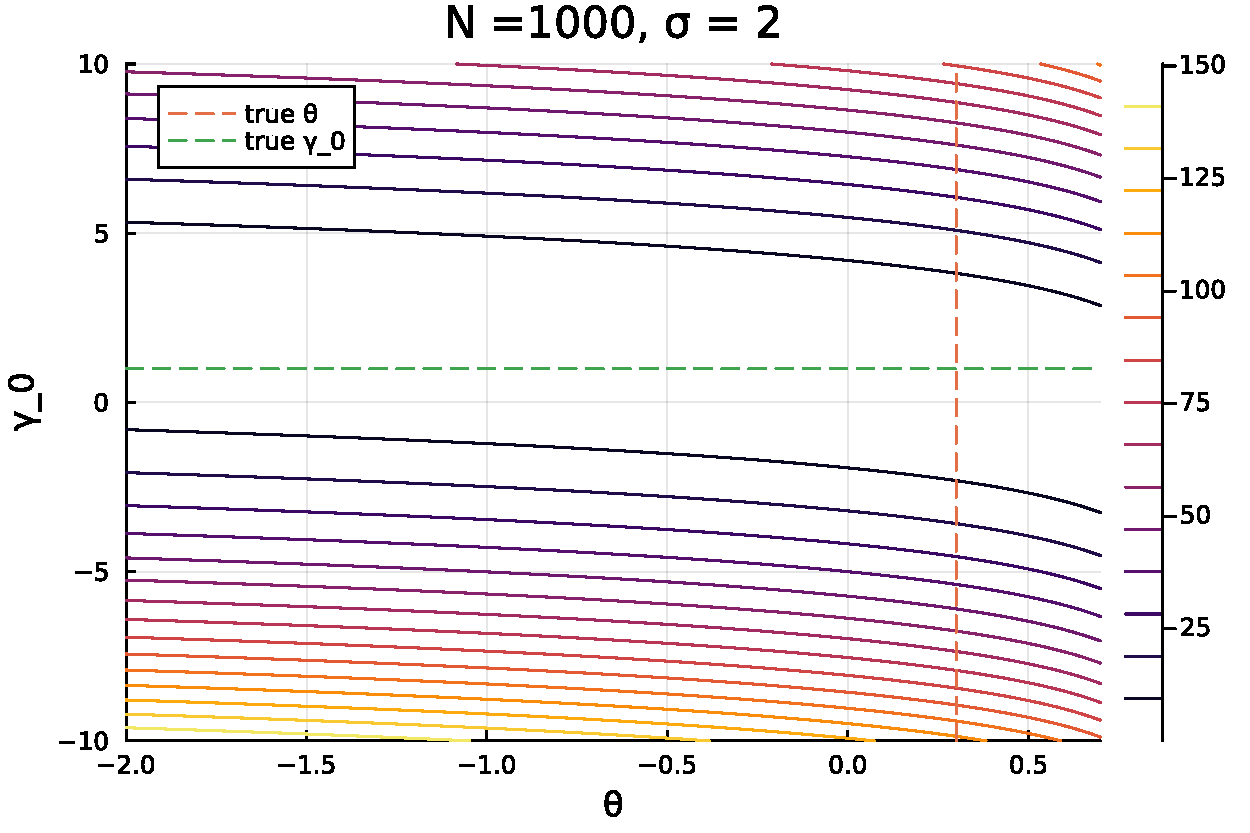
\includegraphics[width = 9cm]{figuretable/contour_loglinear_loglinear_n_1000_sigma_2.pdf}
        \caption{Contour map of the GMM function}
        \label{fig:contour_map}
    \end{figure}
\end{frame}

\begin{frame}{}
    \begin{itemize}
        \item Due to the flat region, the nonlinear solve stops at a point that is far from the true parameter
    \end{itemize}
    \begin{figure}
        \centering
        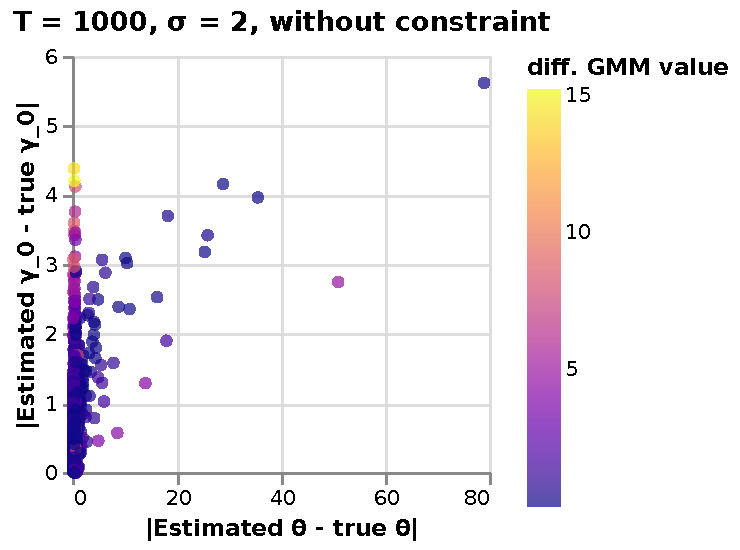
\includegraphics[width = 7cm]{figuretable/diff_gmm_value_loglinear_loglinear_n_1000_sigma_2_non_constraint.pdf}
        \caption{Differece of the GMM under the true parameter and the estimated parameter}
        \label{fig:gmm_diff}
    \end{figure}
\end{frame}


\begin{frame}{}
    \begin{itemize}
        \item As we mentioned, the theoretical range of the conduct parameter is between zero and one
        \item Can putting the constraint on the conduct parameter lead to an accurate result?
        \begin{figure}
            \centering
            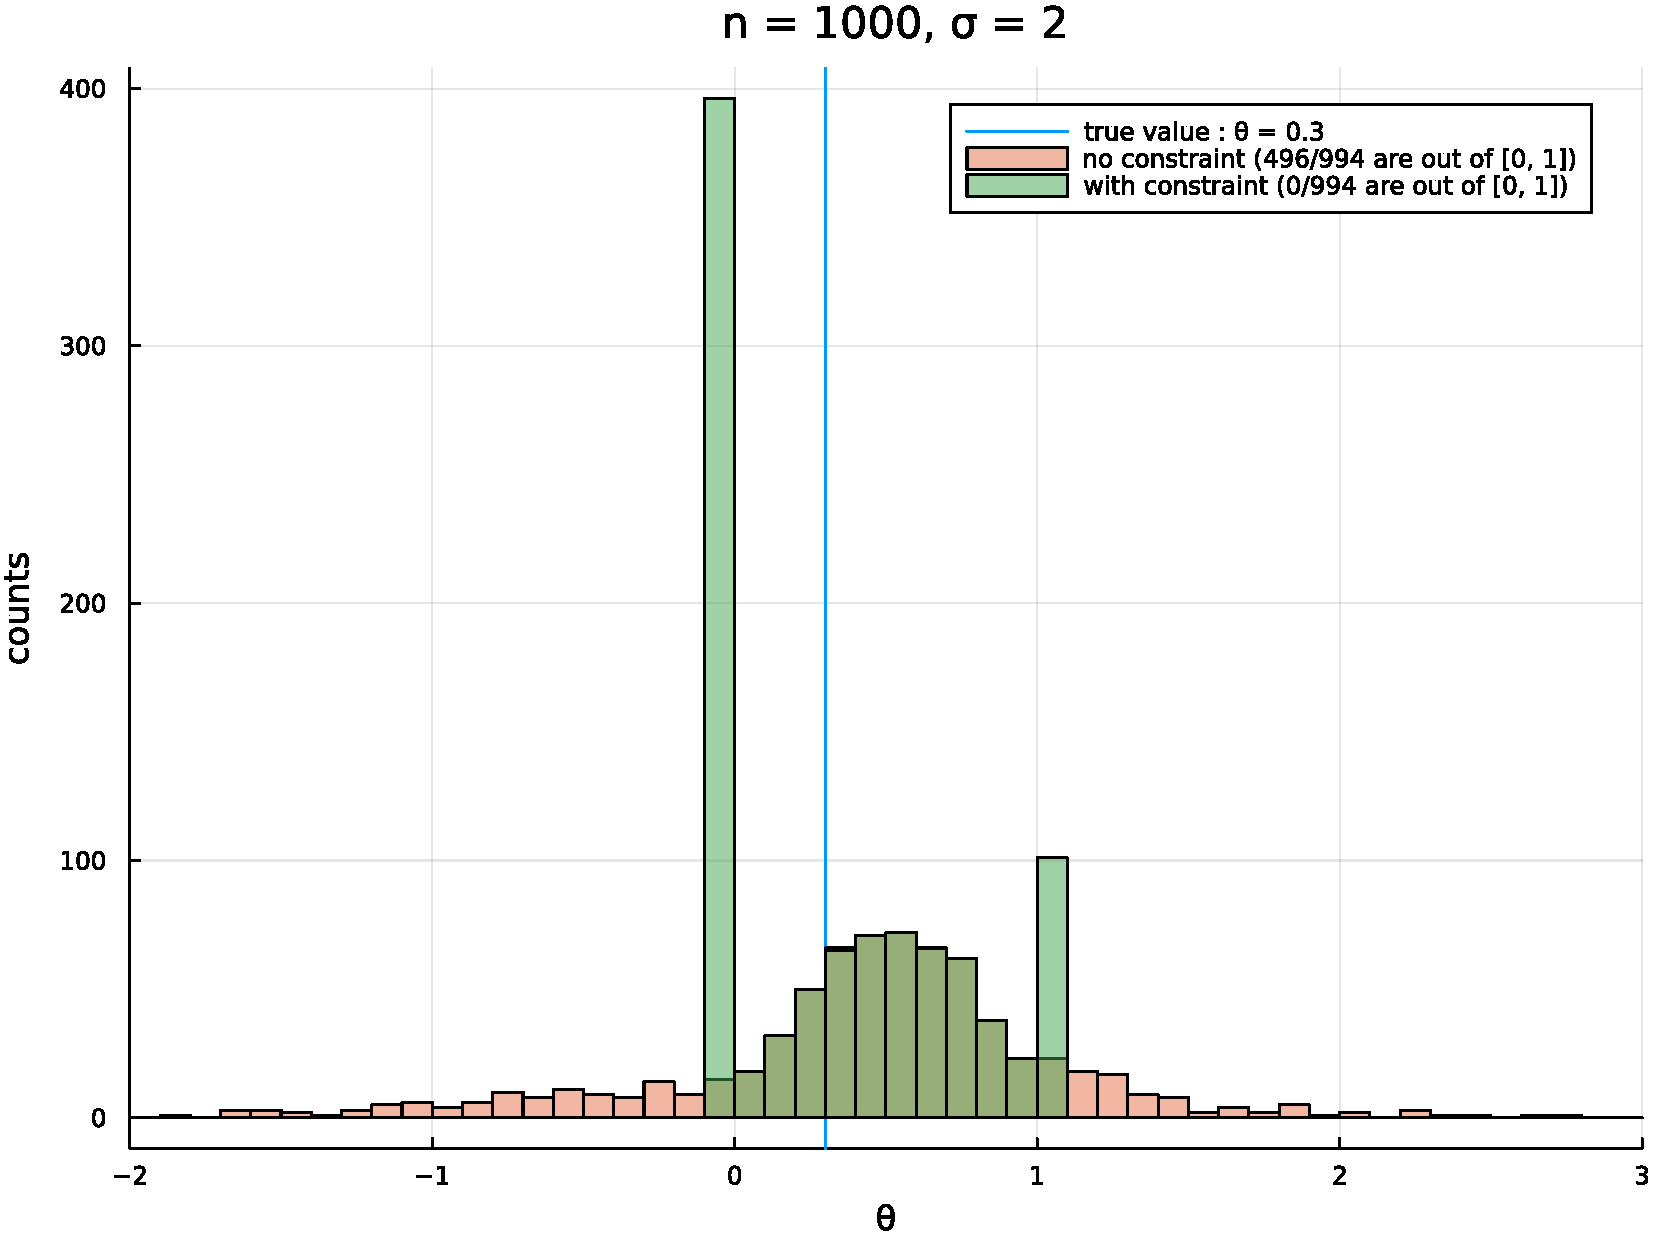
\includegraphics[width = 7cm]{figuretable/histogram_loglinear_loglinear_n_1000_sigma_2_theta_constraint.pdf}
            \caption{Histogram of the estimated parameter}
            \label{fig:histogram_theta  }
        \end{figure}
    \end{itemize}
\end{frame}


\begin{frame}{Summary}
    \begin{itemize}
        \item We reinvestige the conduct parameter estimation in homogeneous product markets
        \item Unlike the conclusion in Perloff and Shen (2012), we find that the conduct parameter estimation in homogeneous product markets with the linear model can lead to accurate results
        \item While Perloff and Shen (2012) suggest using the log-linear model, we find the model is suffered from other estimation problems
    \end{itemize}
\end{frame}


\end{document}